\documentclass{article}
\usepackage[utf8]{inputenc}
\usepackage{latexsym}
\usepackage{url}
\usepackage{hyperref}
\usepackage{graphicx}
\usepackage[table]{xcolor}
\usepackage[T1]{fontenc} 
\usepackage{LobsterTwo}
\usepackage{amsmath} %for math operations
\usepackage{fancyhdr} %for page style
\usepackage{lastpage} %for no of page
\usepackage[a4paper, total={6in, 8in}]{geometry} %for margins
\usepackage{geometry}
\geometry{right=24mm,left=24mm,top=45mm,bottom=45mm} %for page size 
\usepackage{bookman}
\usepackage{array}
\usepackage{wrapfig}
\usepackage{multirow}
\usepackage{tabularx}
\usepackage{amssymb}
\hypersetup{
     colorlinks=true, % make the links colored
     linkcolor=red,   % make the links colored
     urlcolor=blue    % make the URL colored
    }
    
\usepackage{listings}
\usepackage{color}
\usepackage{graphicx}
\usepackage{setspace}
 
\definecolor{dkgreen}{rgb}{0,0.6,0}
\definecolor{gray}{rgb}{0.5,0.5,0.5}
\definecolor{mauve}{rgb}{0.58,0,0.82}
 
\lstset{frame=tb,
  language=Java,
  aboveskip=3mm,
  belowskip=3mm,
  showstringspaces=false,
  columns=flexible,
  basicstyle={\normalsize\itshape},
  numbers=none,
  numberstyle=\tiny\color{gray},
  keywordstyle=\color{blue},
  commentstyle=\color{dkgreen},
  stringstyle=\color{mauve},
  breaklines=true,
  breakatwhitespace=true
  tabsize=2
}


    
\graphicspath{ {figures/} }
\color{black}
\setlength{\parindent}{4em}
\setlength{\parskip}{1em}
\renewcommand{\baselinestretch}{1}
\pagestyle{fancy}
\fancyhf{}
\rhead{\textcolor{blue}{\bfseries{$\copyright$}} Andreea Drăghici}
\renewcommand{\headrulewidth}{1pt}
\renewcommand{\footrulewidth}{1pt}
\rfoot{\textcolor{blue}{\textbf{Pagina}} \textbf \thepage \hspace{1pt} \textcolor{blue}{\textbf{din}} \pageref{LastPage}}
\renewcommand*\abstractname{\textcolor{red}{Rezumat}}
\renewcommand*\refname{\textcolor{red}{Referinte bibliografice}}
\renewcommand{\figurename}{Figura}
\renewcommand*\contentsname{
    \begin{abstract}
      Acest raport este o introducere in obiectivele de dezvoltare a temei de casa la disciplina Sisteme Concurente si Distribuite.
    \end{abstract}   
    \centering \textcolor{red}{ Introducere cuprins }}
\begin{document}
\slshape
\normalsize
\upshape
\sffamily
\begin{titlepage}
\begin{center}
    \textcolor{blue}{\textsc{\huge\scshape\textbf{RAPORT TEHNIC }}}\\[1cm]
    \vspace{20mm}
    \textbf{Universitatea din Craiova,\ Facultatea de Automatică, Calculatoare și Electronică}\\
    \vspace{7mm}
    \textbf{\includegraphics[scale=0.4]{logo-ace.jpg}}
\end{center}
\vspace{3mm}
\begin{center}
\textcolor{blue}{\textsc{\huge\itshape{Sisteme Concurente si Distribuite}}}\\[1.5cm]
	    \vspace{10mm}
	\end{center}
	\begin{minipage}{1\textwidth}
			\Large
			  \textcolor{blue}{\itshape\textbf{Student}} : \itshape{Drăghici Andreea-Maria}\\[0.5cm] 
			  \textcolor{blue}{\textbf{Grupa}} : \itshape{CR 3.1 B}\\[0.5cm] 
			  \textcolor{blue}{\textbf{Anul de studiu}} : \itshape{III}\\[0.5cm] 
			  \textcolor{blue}{\itshape{}\textbf{Specializarea}} : \itshape{Calculatoare Română}\\[2cm]
			  \begin{center}
			      \centering\textcolor{black}{\textbf{$\blacktriangleleft$ Ianuarie 2022 $\blacktriangleright$}}
			  \end{center}
	\end{minipage}
\end{titlepage}
\tableofcontents
\newpage
	\begin{center}
	  \textcolor{blue}{\section{\bfseries\scshape\textcolor{blue}{Contextul problemei}}}
	   \vspace{3mm}
	\end{center}

\textcolor{blue}{\subsection{\itshape  \textcolor{blue}{Cerinta }}}
 \quad Craciunul se apropie! Mos Craciun si angajatii sai (elfii si renii) se pregatesc pentru un nou Craciun care aduce bucurie si cadouri tuturor copiilor din jurul lumii. El este proprietarul unui atelier care contine mai multe fabrici (in fiecare an el reconstruieste fabricile).\\
Angajatii sunt elfii care construiesc jucarii, renii care asteapta sa impacheteze jucariile sub forma de
cadouri.\\ Mos Craciun are nevoie disperata ca atelierul sa functioneze, tinand cont ca ultimul manager
batran al atelierului a plecat. Planul atelierului contine reguli care ne asigura ca toate cadourile sunt
create la timp astfel incat nici un copil sa nu ramana fara darul de Craciun.\\
Mos Craciun doreste sa-l ajuti la implementarea planului fabricii utilizand concurenta in Java (el stie ca
esti expert in acest domeniu).\par	
\vspace{3mm}

\textcolor{blue}{\subsection{\itshape \textcolor{blue}{Indicatii }}}	
Mos Craciun stie ca avem la dispozitie urmatoarele instrumente utile de
programare concurenta:
\begin{itemize}
    \item Semafoare, monitoare si zavoare
    \item Fire de executie. Fiecare elf poate fi reprezentat de un fir separate de executie in cadrul planului
atelierului
    \item Ele trebuie sa comunice: elfii creaza cadouri si renii le primesc pentru a le transmite lui Mos Craciun
    \item Mos Craciun vrea ca renii sa-I transmita cadourile prin TCP/IP, pentru a nu se pierde nici un cadou.
care le va livra copiilor.
\end{itemize}

\newpage
    \begin{center}
	    \textcolor{blue}{\section{\bfseries\scshape\textcolor{blue} {Explicatia rezolvarii alese }}}
	   \vspace{10mm}
	\end{center}
	
    \begin{center}
        \textsc{\Huge \textbf{\itshape Programare concurenta}}\\[0.2cm]
         \vspace{5mm}
    \end{center}
\textcolor{blue}{\subsection{\itshape \textcolor{blue}{Descrierea si intelegerea problemei }}}
\vspace{5mm}    
Cunoastem ca Mos Craciun detine mai multe fabrici de jucarii. Fiecare fabrica contine elfi ce sunt creati aleator si ocupa o pozitie aleatoare in fabrica, la un moment aleator de timp, de aici deducem ca fabrica are o dispunere matriciala de forma N \emph X N, deci nu pot exista mai mult de N \emph / 2 elfi.\\\\
Elfii creaza cadouri mutandu-se intr-una din directiile: stanga, dreapta, sus, jos, iar la fiecare mutare ei creaza un cadou. Deducem ca aceste cadouri trebuie sa fie transmise lui Mos Craciun cu ajutorul renilor, renii asteapta sa primeasac cadouri de la fabrici si sa le trimeata printr-o conducta catre Mos Craciun.\\\\
\textbf{Concluzia: } Atelierul lui Mos Craciun trebuie sa contina toate fabricile, sa le creeze si sa creeze elfii aleator in fabrici.

\vspace{5mm}
\textcolor{blue}{\subsection{\itshape \textcolor{blue}{ Abordarea  problemei }}}
\vspace{5mm}
In opinia mea, fiecare indicatie si instructiune enumerata atat mai sus, cat si in fisierul pdf de pe classroom, pot sa fie privite ca niste clase ce contin ca metode si date explicatiile insiruite.\\\\
In imaginea de mai jos se poate vedea ahitectura claselor. Mai multe detalii vor fi prezentate in sectiunea: Proiectarea Aplicatiei.

\begin{figure}
   \centering
   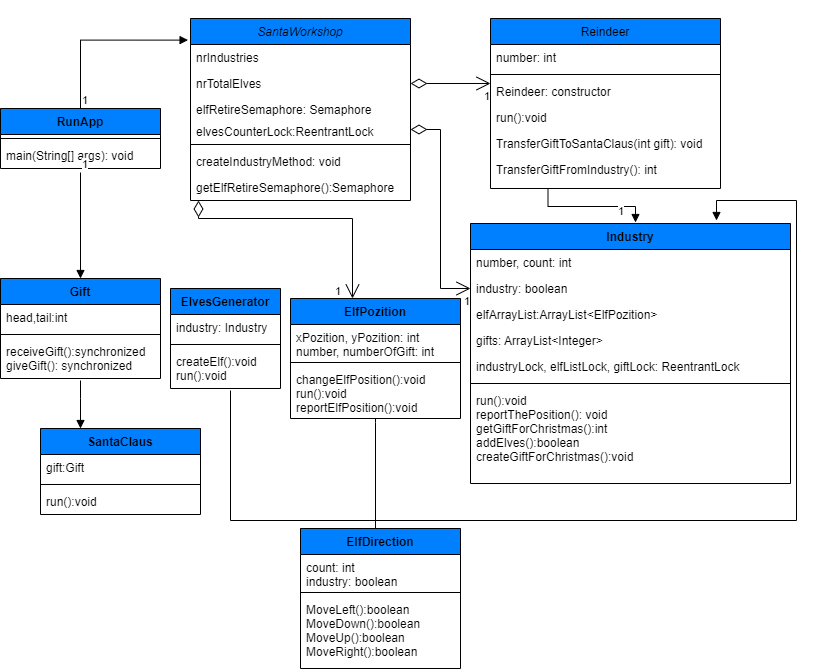
\includegraphics[width=14cm, height=10cm]{Arhitecture.png}
   \bfseries\caption{\textbf{\textcolor{blue}{Arhitectura claselor}}}
\end{figure}


\newpage

\begin{center}
     \textcolor{blue}{\section{\bfseries\scshape\textcolor{blue}{Date experimentale}}}
\end{center}

Data de intrare vor fi generate aleatoru. O instanta a clasei Random in Java va fi folosita pentru a genera un flux de numere pseudoaleatoare.\\ \newline
Vom genera aleatoru fabricile(intre 2 si 5 fabrici). O fabrica creaza jucarii, nu stim numarul jucariilor necesare pana in momentul in care planul fabricii este creat si executat.\\\newline Toate fabricile au o dispunere matriciala de forma N X N, unde N este un numar aleator intre 100-500. In cazul nostru N este redat de variabila number.\\

\begin{lstlisting}
  public void createIndustryMethod() {

        Random rand = new Random();
        nrIndustries = rand.nextInt(4) + 2;
        int nrReindeers = rand.nextInt(10) + 8;
        industries = new Industry[nrIndustries];
        generators = new ElvesGenerator[nrIndustries];
        reindeers = new Reindeer[nrReindeers];

        List<String> asList = Arrays.asList(MessageFormat.format("Au fost create {0} fabrici", nrIndustries), MessageFormat.format("Au fost creati {0} reni", nrReindeers));
        for (int i = 0; i < asList.size(); i++) {
            String s = asList.get(i);
            System.out.println(s);
        }
        IntStream.range(0, nrIndustries).forEachOrdered(i -> {
            int number = rand.nextInt(500) + 100;
            industries[i] = new Industry(number, i + 1);
            generators[i] = new ElvesGenerator(industries[i]);
            System.out.println(MessageFormat.format("Fabrica {0} are {1} elfi",
                    i + 1,
                    number));
        });
        IntStream.range(0, nrReindeers).forEachOrdered(i -> {
            reindeers[i] = new Reindeer(industries, i + 1, giftQueue);
        });
        IntStream.range(0, nrIndustries).forEachOrdered(i -> {
            generators[i].start();
            industries[i].start();
        });
    }
\end{lstlisting}
\vspace{2cm}

Elfii sunt creati si ei aleator in fiecare fabrica intr-o pozitie aleatoare, la un moment aleator de timp.\\\\ Imediat dupa create, fiecare elf creat trebuie sa informeze fabrica despre existenta lui. \\\\ Cunoastem ca nu pot exista mai mult de N/2 elfi in fabrica, deci numarul de elfi va fi mai mic decat dimensiunea fabricii.\\\\
\newline

\begin{lstlisting}
 public void createElf() {
 
        Random rand = new Random();
        ReentrantLock factoryLock = industry.getFactoryLock();
        // elfii nu se pot misca in timp ce in fabrica este adugat un nou elf
        factoryLock.lock();
        
        var industryCount = industry.getCount();
        if (industry.numberOfElves() == (industryCount / 2)) {
            factoryLock.unlock();
            
        } else {
        
            var X = rand.nextInt(industryCount);
            var Y = rand.nextInt(industryCount);
            ReentrantLock elvesCounterLock = getElvesCounterLock();
            
            //niciun alt fir nu poate accesa nr de elfi din fabrica
            //acesta este modificat acum
            elvesCounterLock.lock();
            // creaza un nou elf
            ElfPozition elf = new ElfPozition(nrTotalElves, X, Y, industry);
            
            // adauga elfii in fabrica
            if (industry.addElves(elf)) {
                nrTotalElves += 1;
                
                System.out.println(MessageFormat.format("Elful cu numarul {0} a fost creat in fabrica {1} cu succes ",
                        elf.getNumber(),
                        industry.getNumber()));
                        
                elvesCounterLock.unlock();
            } else {
                elvesCounterLock.unlock();
            }
            factoryLock.unlock();
        }
\end{lstlisting}

\newpage   
\begin{center}
     \textcolor{blue}{\section{\bfseries\scshape\textcolor{blue}{Proiectarea aplicatiei}}}
\end{center}
\vspace{10mm}
 \textcolor{blue}{\subsection{\itshape \textcolor{blue}{Structura de nivel inalt a aplicatiei }}}
\vspace{15mm}
Aplicatia este alcatuita din pachete ce contin subpachete, respectiv clase. Fiecare clasa este organizata avand membrii si functii membre.\\ Pentru rezolvarea temei de casa am folosit notiunile acumulate din platformele de laborator, cat si indicatiile din assignment.\\\\
\textcolor{red}{\bfseries Implementarea contine un singur pachet, acesta avand mai multe subpachete:}
\begin{itemize}
    \item \textbf{com.tema.home} - pachetul principal;
    \item \textbf{initialiplementation} - subpachetul ce contine implementarea initiala;
    \item \textbf{cyclicbarrier} - subpachetul ce contine implementarea utilizand bariere;
    \item \textbf{semaphores} - subpachetul ce contine implemenatrea utilizand semafoare;
\end{itemize}
\begin{figure}
   \centering
   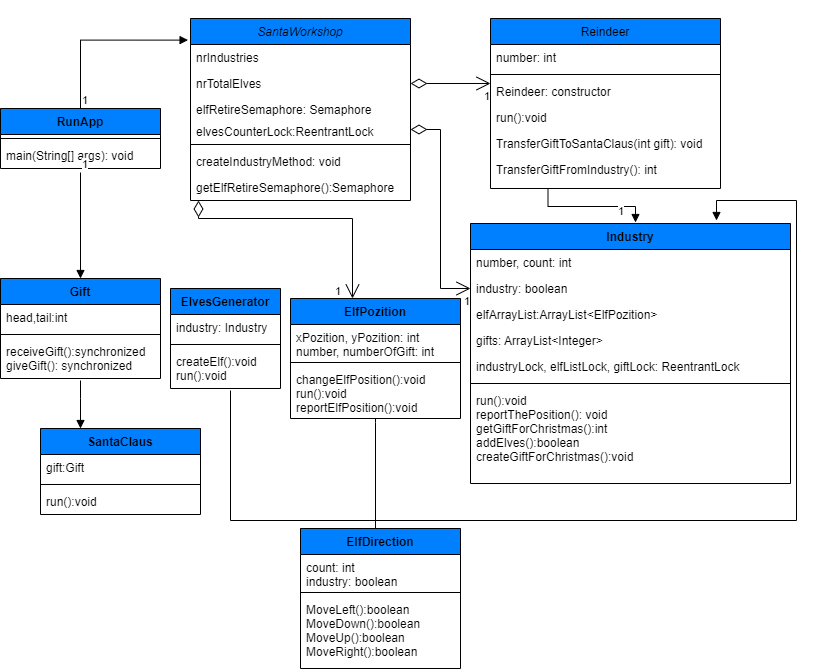
\includegraphics[width=14cm, height=14cm]{Arhitecture.png}
   \bfseries\caption{\textbf{\textcolor{blue}{Arhitectura claselor}}}
\end{figure}
Primul subpachet reprezinta implementarea initiala, cea generica pentru tema nostra de casa.\\\\ Cel de al doilea subpachet reprezinta rezolvarea problemei utilizand Cyclic Barrier, unde am rescris implemenatrea cu odihnirea elfilor folosind aceasta clasa.\\\\
Cel de al treilea subpachet cuprinde rezolvarea problemei utilizand semafoare.
Am ales aceasta abordare pentru a avea la final o structura cat mai organizata ce incearca sa atinga fiecare task din assignment.\\\\
Imaginea atasata constituie diagrama UML unde am incercat sa scot in evidenta structura claselor.\\\\ Fiecare clasa contine metode ce ajuta la rezolvarea problemei. O parte din clase sunt instantiate in fisierul RunApp, ce reprezinta fisierul principal ce ruleaza programul.\\\\ Cum spuneam si mai devreme, fiecare instructiune din assignment a fost transpusa in cate o clasa, respectiv metoda, mai jos se poate vedea acest lucru.
\vspace{7mm}
\newpage
\textcolor{blue}{\subsection{\itshape \textcolor{blue}{Specificatia formatului datelor de intrare}}}
\vspace{7mm}
Datele de intrare sunt generate aleatoriu folosind o instanta a clasei Random pentru a genera un flux de numere pseudoaleatoare.\\\\
Generam aleatoriu fabricile, fabricile avand o dispunere matriceala N \emph{X} N, iar N este aleatoriu intre 100 si 500.\\Elfii sunt creati si ei aleator in fiecare fabrica intr-o pozitie aleatoare, intr-un anumit timp.
\vspace{7mm}
\textcolor{blue}{\subsection{\itshape \textcolor{blue}{Specificatia formatului datelor de iesire}}}
\vspace{7mm}
Datele de iesire vor reprezenta numarul de fabrici, numarul de reni,numarul de elfi, cat si pozitia elfilor in fabrica.\\
\textcolor{blue}{\subsection{\itshape \textcolor{blue}{Lista tuturor modulelor aplicatiei si descrierea lor}}}
\vspace{7mm}
Clasa \textbf{ElfDirection} cuprinde implemenatarea pentru a verifica in care dintre directiile stanga, dreapta, sus, jos se poate muta un elf cand creaza cadouri.
Pentru a verifia fiecare directie de mai sus, am implementat cate o metoda care ne returneaza rezultatul directiei in care elfii se muta.\\\\
Clasa \textbf{ElfPozition} implementeaza doua metode, o metoda care ne ajuta sa schimbam pozitia in care un elf se afla, deoarece doi elfi nu se pot afla in aceeasi pozitie si o metoda care ne afiseaza pozitia fiecarui elf in fabrica.\\
Tot in aceasta clasa intalnim si metoda run() care contine un semafor pe care elfii incearca sa-l achizitioneze pentru a primi permisiunea sa se retraga.\\\\
Clasa \textbf{ElvesGenerator} implementeaza o metoda numita \textbf{createElf} care ne ajuta sa generam elfii intr-o anumita fabrica. (aceasta metoda a fost deja explicata mai sus in descrierea datelor experimentale).\\
Mai implementeaza si metoda run unde firul nostru va realiza urmatoarele actiuni (elfii sunt creati aleator in fiecare fabrica intr-o pozitie aleatoare, la un moment aleator de timp) intr-o bucla infinita.\\\\
Clasa \textbf{Gift} implementeaza doua metode, receiveGifft si giveGift pentru a primi un cadou de la reni si de a tansfera cadourile catre Mos Craciun.\\\\
Clasa \textbf{Industry} implementeaza un fir care actioneaza ca o fabrica. In aceasta clasa mai gasim si o metoda care cere tuturor elfilor existenti pozitia lor actuala, deoarece elfii nu se pot misca in timp ce isi rapoarteaza pozitia, iar renii nu pot primi cadouri in timp ce fabrica le cere elfilor pozitia si in timp ce acestia creeaza un cadou.\\\\
Clasa \textbf{Reindeer} implementeaza un fir ce se comporta ca un ren.\\
Aceasta clasa mai implementeaza inca doua metode, una care ofera cadourile Mosului, punandu-le in coada de cadouri si o alta metoda care ne solicita un cadou existent de la o fabrica aleasa la intamplare.\\\\
Clasa \textbf{SantaClaus} implementeaza un fir ce se comporta ca Mos Craciun. Tot aici gasim implementata si metoda care il ajuta pe Mos Craciun sa primeasca cadouri la nesfarsit.\\\\
Clasa \textbf{SantaWorkshop} reprezinta fix atelierul lui Mos Craciun. Aceasta clasa cuprinde numarul de fabrici existente, numarul total de elfi exitenti, numarul de elfi si o metoda care ne ajuta sa generam fabricile. Aceasta metoda a fost explicata in paragraful Date experimentale.\\\\
Clasa \textbf{RunApp} cuprinde o parte din clase ce sunt instantiate aici, in aceasta clasa  ruleaza programul principal. Se creeaza coada de transfer a cadourilor, il creaza pe Mos Craciun, creeaza atelierul acestuia, apoi atelierul incepe sa creeze fabrici, iar Mos Craciun incepe sa primeasca cadouri de la reni.\newline
\textcolor{blue}{\section{\itshape \textcolor{blue}{Decizia implementarii sarcinilor suplimentare}}}
\textcolor{blue}{\subsection{\itshape\textcolor{blue}{Task 1. Retragerea unui elf}}}
Pentru retragerea unui elf, folosim un semafor pe care elfii incearca sa-l achizitioneze pentru a primi permisiunea sa se retraga. Retragerea unui elf inseamna ca acesta va fi eliminat din fabrica si din lista elfilor exitenti.
\begin{lstlisting}
 public void run() {
        do {
            /* semafor pe care elfii incearca sa-l achizitioneze pentru a primi permisiunea sa se retraga.*/
            getElfRetireSemaphore().release();
            // Sleeping 50 milliseconds
            try {
                Thread.sleep(50);
            } catch (InterruptedException e) {
                extracted(e);
            }
        } while (true);
    }
     /*
     * metoda pentru sarcina suplimentara" retragerea unui elf
     * blocheaza accesul la lista de elfi
     * blocheaza accesul la lista fabricii
     * elimina pozitia elfului din lista fabricii
     * deblocheaza accesul la lista cu elfii
     * deblocheaza accesul la lista fabricii
     */
    public void retireElf(ElfPozition elfPozition) {

        try {
            /* modificarea listei elfilor si a pozitiei matricei fabricii */
            elfListLock.lock();//blocheaza accesul la lista de elfi
            industryLock.lock();//blocheaza accesul la lista fabricii
            elfArrayList.remove(elfPozition);//elimina pozitia elfului din lista fabricii
            int X = elfPozition.getxPozition();
            int Y = elfPozition.getyPozition();
            industry[X][Y] = false;
            System.out.println(MessageFormat.format("Elful cu numarul {0} s-a retras din fabrica cu numarul {1}", elfPozition.getNumber(), number));
        } finally {
            elfListLock.unlock();//deblocheaza accesul la lista cu elfii
            industryLock.unlock();//deblocheaza accesul la lista fabricii
        }
    }
\end{lstlisting}
\textcolor{blue}{\subsection{\itshape\textcolor{blue}{Task 2. Odihnirea unui elf (utilizand semafoare) }}}
Presupunem ca elful va ajunge la diagonala principala si va incerca sa dobandeasca un semafor pentru a modifica contorul pentru elfii ce asteapta la bariera, asteptand pana cand contorul este mai mic ca dimensiunea fabricii. Am modificat programul astfel incat atunci cand elful se afla in zona diagonalei principale acesta se va opri din miscare. Astfel daca toti elfii s-au oprit in zona diagonalei principale, ei vor fi treziti sa-si continue miscarea pana cand or ajunge sa se odihneaza in zona diagonalei principale.\\

\textcolor{blue}{\subsection{\itshape\textcolor{blue}{Task 3. Folosirea clasei CyclicBarrier }}}
Presupunem ca elful va ajunge la diagonala principala si va astepta la bariera pana cand \emph{N} elfi o ating. Am utilizat pachetul java.util.concurrent contine clasa CyclicBarrier, ce furnizeaza o metoda mai convenabila de implementare a sincronizarii la bariera si am rescris programul cu odihnirea elfilor folosind aceasta clasa.

\begin{center}
    \textcolor{blue}{\section{\bfseries\scshape\textcolor{blue}{Observatii si Rezultate}}}
\end{center}
\vspace{10mm}
Pentru sincronizarea intrarii renilor in fabrica am folosit un semafor cu 10 permise pentru fiecare fabrica, adica maxim 10 reni pot accesa in acelasi timp fabrica.\\
\begin{lstlisting}

 //semafor pentru numarul maxim permis de reni in fabrica
 
 private final Semaphore reindeerSemaphore = new Semaphore(10); 
 
\end{lstlisting}
\vspace{5mm}
Pentru transferul cadourilor de la reni catre Mos Craciun a fost folosita o coada concomitenta care sincronizeaza metodele de adaugare a unui cadou in coada si scoaterea unui cadou din coada.
\begin{lstlisting}

 //metoda utilizata de Mos Craciun pentru a primi un cadou de la reni
 
    public synchronized int receiveGift() {
    
        /* asteptam pana cand buffer ul nu mai este gol */
        if (tail == head) {
            do {
                try {
                    wait();
                } catch (InterruptedException e) {
                    extracted(e);
                }
            } while (tail == head);
        }
        /* primire cadou */
        int gift = giftsCount[head % giftsCount.length];
        head += 1;
        
        /* notificati ca buffer ul nu este plin */
        notifyAll();
        
        return gift;
    }


    //metoda utilizata de un ren pentru a transmite un cadou lui Mos Craciun
    
    public synchronized void giveGift(int gift) {
    
        if (tail - head == giftsCount.length) {
            do {
                try {
                    wait();
                } catch (InterruptedException e) {
                    extracted(e);
                }
            } while (tail - head == giftsCount.length);
        }
        giftsCount[tail % giftsCount.length] = gift;
        
        /* adaugare cadou */
        tail += 1;
        notifyAll();
    }
\end{lstlisting}
\vspace{5mm}
Pentru funtionarea corecta a fabricilor am utilizat 3 incuietori.\\\\

\begin{lstlisting}

    //blocarea accesarii fabricii
    private final ReentrantLock industryLock = new ReentrantLock();
    
    //un lacat pentru accesarea listei de elfi
    private final ReentrantLock elfListLock = new ReentrantLock();
    
    //un lacat pentru accesarea listei de cadouri
    private final ReentrantLock giftLock = new ReentrantLock();
    
\end{lstlisting}
\vspace{5mm}
Stim ca doi elfi nu se pot deplasa in acelasi timp in fabrica sau doi elfi nu se pot misca in timp ce isi raporteaza pozitia.\\ \newline
Doi elfi nu pot fi adaugati in acelasi timp in lista de elfi, lista nu poate fi modificata cand doi elfi isi raporteaza pozitia.\\  \newline
Un ren nu poate primi un cadou in timp ce fabrica le cere elfilor sa-si raporteze pozitia. Lista de cadouri a unei fabrici poate fi accesata de un singur ren la un moment dat.\\

In aceasta sectiune voi descrie printr-un mic rezumat rezultatele obtinute in urma rularii programului. Rezultatele sunt obtinute aleatoriu in functie de generarea datelor de intrare.\\\\
Datele de iesire vor reprezenta numarul de fabrici, numarul de reni, numarul de elfi, catsi pozitia elfilor in fabrica. Rezultatele obtinute in urma rularii programului sunt cele de mai sus.
\begin{figure}
      \centering
      \includegraphics[width=10cm]{exempluOutput.jpg}
      \bfseries\caption{\textbf{\textcolor{blue}{Output}}}
\end{figure}
\newpage 
\begin{center}
    \textcolor{blue}{\section{\bfseries\scshape\textcolor{blue}{Concluzii si Bibliografie}}}
\end{center}
\begin{itemize}
    \item Consider ca aceasta tema a reprezentat o provocare, atat intelegerea cerintei, abordarea task-urilor, cat si implementarea.
    \vspace{2mm}
    \item In urma acestei teme, mi-am imbunatatit abilitatile de coding in limbajul Java, cat si notiunile de sintaxa in LaTex.
    \vspace{2mm}
    \item O alta concluzie este reprezentata de termenul limita al temei de casa. Acest parametru a avut un impact mai bun asupra organizarii timpului, cat si asupra unei coordonari mai responsabile a celorlalte aspecte realizate pentru a rezolva aceasta tema, ceea ce constituie un beneficiu mai amplu pentru dezvoltarea mea in acest domeniu.
       \vspace{2mm}
\end{itemize}
\begin{flushleft}
Mai jos se pot observa cateva referinte bibliografice, capitole din cursuri, carti, site-uri web, referinte ce au ajutat in parcurgerea, documentarea si intelegerea mai ampla a temei de casa. \\\\
De pe site-urile respective m-am documentat, link-urile sunt atasate mai jos: 
\begin{thebibliography}{8}
\bfseries\scshape
        \bibitem{java} 
        Java concurrency (multi-threading) - Tutorial,
        \textcolor{blue}{\\\url{https://www.vogella.com/tutorials/JavaConcurrency/article.html}}
        \bibitem{gfg} 
         Reentrant Lock in Java,
        \textcolor{blue}{\\\url{https://www.geeksforgeeks.org/reentrant-lock-java/}}
        \\\url{}
        \bibitem{gfg} 
         Semaphore in Java,
        \textcolor{blue}{\\\url{https://www.geeksforgeeks.org/semaphore-in-java/}}
        \\\url{https://docs.oracle.com/javase/7/docs/api/java/util/concurrent/Semaphore.html}
        \bibitem{locks} 
         Java 8 Concurrency Tutorial: Synchronization and Locks,
        \textcolor{blue}{\\\url{https://winterbe.com/posts/2015/04/30/java8-concurrency-tutorial-synchronized-locks-examples/}}
          \bibitem{CyclicBarrier} 
         Java.util.concurrent.CyclicBarrier in Java,
        \textcolor{blue}{\\\url{https://www.geeksforgeeks.org/java-util-concurrent-cyclicbarrier-java/}}
        \\\url{https://docs.oracle.com/javase/7/docs/api/java/util/concurrent/CyclicBarrier.html}
        \\\url{https://www.javatpoint.com/lock-in-java}
        \bibitem{overleafwebsite} 
        Introducing Overleaf and LaTeX,
        \textcolor{blue}{\\\url{https://www.overleaf.com/learn/latex/Tutorials}
        \\\url{https://oeis.org/wiki/List_of_LaTeX_mathematical_symbols}
        \\\url{https://mirrors.nxthost.com/ctan/macros/latex/required/graphics/grfguide.pdf}
        \\\url{https://sharelatex.psi.ch/learn/XeLaTeX}}
        \bibitem{capitol-curs} 
         Capitolul 12 din curs, cat si restul cursurilor de pe classroom.\\
        \bibitem{laborator}
         Laborator 12, cat si restul laboratoarelor de pe classroom.
\end{thebibliography}
\large \textcolor{blue}{\bfseries{$\copyright$}} Ianuarie 2022.
\end{flushleft}

\end{document}
